\problemname{Collect Stones}

$N$ stones are lying scattered in a coordinate system. Each stone has a coordinate ($x_i$,$y_i$). It is time to collect the stones, and to help you have acquired a super-smart stone-collecting machine.

Before the machine starts, you choose a point that you call the collection point $S$. It is the point where the machine starts and where it will place the collected stones. It must be somewhere on the x-axis. The machine starts at the collection point $(S,0)$, and then collects all stones and places them at the collection point. The machine can only carry \emph{one stone at a time}.

Fuel is expensive, so you thought you would try to be a bit smart. You know that when the machine starts, it always collects all stones optimally, but it is up to you to choose the collection point so that the total distance traveled by the machine is minimized. How long is this distance, given that you choose the collection point optimally? You can consider the stones and the machine as points in the plane.

\section*{Input}
The first line contains the integer $N$ ($1 \leq N \leq 10^5$), the number of stones.

Then follow $N$ lines with pairs of floating-point numbers $x_i$ $y_i$, the coordinates of the stones. All stones in
the input are at most 100 distance units from the origin.

\section*{Output}
Output a number: the minimum possible total distance traveled by the machine after collecting all stones. An absolute error less than $10^{-4}$ is considered correct.

{\bf Tip:} Make sure your program outputs enough decimal places even when the answer is large.

\section*{Scoring}
Your solution will be tested on a set of test groups.
To earn points for a group, you must pass all test cases in that group.

\noindent
\begin{tabular}{| l | l | p{12cm} |}
  \hline
  \textbf{Group} & \textbf{Points} & \textbf{Constraints} \\ \hline
  $1$    & $30$       & All stones lie on the x-axis and $N \leq 1000$. \\ \hline
  $2$    & $30$       & All stones lie on the x-axis. \\ \hline
  $3$    & $40$       & No additional constraints. \\ \hline
\end{tabular}


\section*{Explanation of Sample 1}

\begin{figure}[!h]
\begin{center}
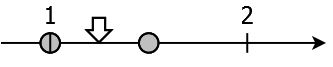
\includegraphics[scale=0.4]{stenar1.png}
\end{center}
\caption{The figure shows a possible choice of starting point that leads to minimal travel distance for the machine, x = 1.25. The machine needs to travel 0.5 distance units to fetch the left stone, and then 0.5 distance units to fetch the right stone.}
\label{fig1}
\end{figure}

\section*{Explanation of Sample 2}
\begin{figure}[!h]
\begin{center}
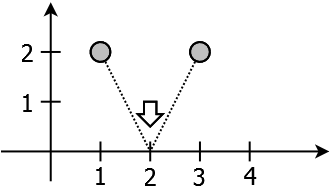
\includegraphics[scale=0.4]{stenar2.png}
\end{center}
\caption{The figure shows the optimal starting position for the machine, at x = 2.0. Total distance traveled is $4\cdot\sqrt{2^2 + 1} = 8.94427191...$ .}
\label{fig1}
\end{figure}
